
\chapter*{Clustering}

    \subsection*{Why do clustering?}
    
        In chapter 4, we discussed \textbf{classification}: sorting data points into different groups, or \textbf{classes}. 
        
        \miniex We might sort animals by \textbf{genetics}, or different sub-diseases that need different \textbf{treatments}. 
        
        \textbf{Simplifying} our data into \textbf{categories} can allow us to do better work, more easily.
        
        This had lots of benefits: 
        
        \begin{itemize}
            \item It could be used to make \textbf{decisions}. For example, a binary classifier could be used to decide "yes" or "no". 
        
            \item We could use this to understand the item It could be used to make yes or no decisions. and \textbf{distribution} of our data.
            
            \item We could sort different types of data to be processed \textbf{separately}.
        \end{itemize}
        
        The problem is, this relied on us \textbf{knowing} what classes we plan to sort into. 
        
        This may seem obvious, but what if we're looking at something \textbf{new}? A disease we don't fully \textbf{understand}, or animals we've never \textbf{seen} before? How do we classify them?
        
        In the past, doing this ourselves has given rise to many of the \textbf{classes} we use to sort things today. But, computers allow us to do this in situations we \textbf{never} could before:
        
        \begin{itemize}
            \item \textbf{High-dimensional} datasets, with too much \textbf{complex} information for a human to make sense of.
            
            \item Discovering new classes \textbf{faster} than ever using computers.
            
            \item Finding \textbf{patterns} in creative ways humans would never think to, especially for really \textbf{abstract} problems.\\
        \end{itemize}
    
        \begin{concept}
            \vocab{Clustering} is like \purp{classification}, where we want to assign things to \gren{classes}: we call them \vocab{clusters}.
            
            But, we use it when we \purp{don't know} what groupings we want, so we have to \gren{find} them.
        \end{concept}
        
        We have some challenges ahead of us, though. Not only do we need to create \textbf{new classes}, we \textit{still} need to classify our points based on them!

%\pagebreak
%%%%%%%%%%%%%%%%%%%%%%%%%%%%%%%%%%%%%%%%%%%%%%%%%%%%%%%%%%%%%%%%%%%%%%%%%%%%%

\section*{Clustering Formalisms}

    \subsection*{Unsupervised Learning}
        
        The first thing we should note: 
        
        This problem is similar to classification, a \textbf{supervised} problem.
        
        It was \textbf{supervised} because we knew the \textbf{correct} labels for our data in our advance. We just wanted to \textbf{teach} it to our computer.
        
        The problem here: we \textbf{don't} know the correct labels! In fact, we're making them up as we go. Because we aren't being "supervised" by a correct answer, we call this \textbf{unsupervised learning}.\\
        
        \begin{concept}
            \vocab{Clustering} is a type of \purp{unsupervised learning}: meaning, we don't have a \gren{correct} answer in advance.
            
            The labels we create are not based on a \purp{known} truth.
            
            The \gren{label} for data point $\ex{x}{i}$ is written as $\ex{y}{i}$.
        \end{concept}
        
    \subsection*{What is clustering?}
    
        So, if we don't know \textbf{what} our classes are, how do we figure out \textbf{which} classes to create?
        
        Intuitively, we think of classes as a \textbf{collection} of things that are \textbf{similar} to each other. Before, we've considered things "\textbf{close}" if they have a \textbf{low distance} in input space.
            \note{Remember that input space is where we represent each data point using input variables.}
            
        \miniex We can tell two animals are \textbf{both} cats because they both have fur and sharp claws, among other things: they're \textbf{similar}.
            
        Meanwhile, two points in different classes are more \textbf{different}: they're further apart in input space. 
        
        \miniex We can tell a dolphin is \textbf{distinct} from a cat because one lives in water and one doesn't: their clusters are more \textbf{different}.
        
        We call each of these groupings \textbf{clusters}.\\
        
        \begin{definition}
            Informally, a \vocab{cluster} is a collection of \gren{data points} that are all 
            \begin{itemize}
                \item \purp{Near} each other
                
                \item \purp{Far} from the other clusters.
            \end{itemize}
            
            We use clusters as our way to \gren{discover} new classifications.
        \end{definition}
        
        \miniex Below, we can visually mark out what looks like 5 distinct \textbf{clusters} in input space $(x_1,x_2) \in \RR^2$:
        
        \begin{figure}[H]
            \centering
            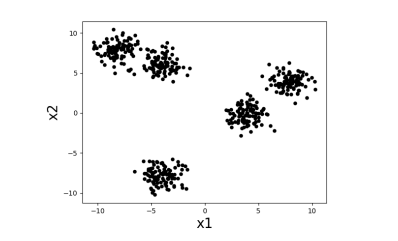
\includegraphics[width=70mm,scale=0.4]{images/clustering_images/clustering_example.png}
        \end{figure}
        
        This is an informal way to understand clusters, though. If we want to be more precise, we need to ask ourselves questions like:
        
        \begin{itemize}
            \item What does it mean for points to be "close" or "far"? How are we measuring distance?
            
            \item How many clusters do we want?
            
            \item How do we evaluate our clustering?
        \end{itemize}
        